\newcommand{\RowsNominal}{%
\midrule\multicolumn{11}{@{}l}{\textbf{MBTA-111 (data-informed simulation)}} \\
\midrule
Fixed-NoHold & $1147.24 \pm 0.00$ & 215.28 & 931.96 & 0.0606 & 0.0605 & 10.74 & 0.28 & 0.00 & 0.007 & $-14.32\ [-21.80,\,-8.21]$ \\
Forward-Hold & $1215.05 \pm 0.00$ & 219.47 & 995.58 & 0.0196 & 0.0196 & 3.73 & 1.61 & 197.28 & 0.007 & $-82.12\ [-91.80,\,-73.59]$ \\
Bilateral-Hold & $1178.26 \pm 0.00$ & 216.09 & 962.17 & 0.0299 & 0.0298 & 5.23 & 0.48 & 80.09 & 0.007 & $-45.34\ [-53.74,\,-38.20]$ \\
Rolling-Heuristic & $1127.72 \pm 0.00$ & 197.76 & 929.96 & 0.0987 & 0.0823 & 12.46 & 10.06 & 5.14 & 0.000 & $+5.20\ [+1.93,\,+8.76]$ \\
Flat-SAC & $1147.69 \pm 0.13$ & 215.22 & 932.47 & 0.0576 & 0.0575 & 10.20 & 0.28 & 5.93 & 0.007 & $-14.77\ [-22.41,\,-8.42]$ \\
NoFreq-HRL & $1142.51 \pm 7.34$ & 207.89 & 934.62 & 0.0759 & 0.0602 & 10.99 & 1.38 & 4.82 & 0.000 & $-9.59\ [-14.25,\,-5.50]$ \\
RawHistory & $1135.70 \pm 2.61$ & 203.08 & 932.62 & 0.0732 & 0.0615 & 11.10 & 1.46 & 4.12 & 0.000 & $-2.78\ [-6.86,\,+0.99]$ \\
AllBand & $1136.05 \pm 3.51$ & 203.18 & 932.87 & 0.0758 & 0.0626 & 11.12 & 2.46 & 3.68 & 0.000 & $-3.13\ [-6.68,\,+1.54]$ \\
Swapped & $1135.05 \pm 3.88$ & 202.34 & 932.71 & 0.0770 & 0.0630 & 11.43 & 3.11 & 5.90 & 0.000 & $-2.13\ [-5.98,\,+1.84]$ \\
NoBudget & $1137.58 \pm 5.88$ & 204.57 & 933.01 & 0.0697 & 0.0584 & 10.38 & 0.53 & 3.74 & 0.000 & $-4.66\ [-12.51,\,+2.46]$ \\
NoPromotion & $1132.71 \pm 2.22$ & 200.85 & 931.86 & 0.0798 & 0.0670 & 11.78 & 6.50 & 4.66 & 0.000 & $+0.21\ [-2.81,\,+3.93]$ \\
FreqDuet & $1132.92 \pm 3.06$ & 201.35 & 931.57 & 0.0739 & 0.0613 & 10.69 & 0.91 & 3.64 & 0.000 & -- \\
\midrule\multicolumn{11}{@{}l}{\textbf{Tidal-Bimodal (synthetic simulation)}} \\
\midrule
Fixed-NoHold & $848.29 \pm 0.00$ & 233.30 & 614.99 & 0.0525 & 0.0524 & 9.31 & 0.24 & 0.00 & 0.009 & $-14.02\ [-29.54,\,+3.95]$ \\
Forward-Hold & $896.56 \pm 0.00$ & 227.26 & 669.30 & 0.0124 & 0.0124 & 2.55 & 1.12 & 172.69 & 0.009 & $-62.29\ [-77.98,\,-44.44]$ \\
Bilateral-Hold & $883.05 \pm 0.00$ & 229.26 & 653.79 & 0.0205 & 0.0204 & 3.54 & 0.54 & 112.55 & 0.009 & $-48.78\ [-64.27,\,-30.92]$ \\
Rolling-Heuristic & $817.95 \pm 0.00$ & 204.24 & 613.71 & 0.1366 & 0.1419 & 18.12 & 33.27 & 3.06 & 0.000 & $+16.32\ [+1.27,\,+36.04]$ \\
Flat-SAC & $848.09 \pm 0.10$ & 232.76 & 615.33 & 0.0504 & 0.0503 & 8.94 & 0.25 & 5.79 & 0.009 & $-13.82\ [-29.26,\,+4.11]$ \\
NoFreq-HRL & $826.03 \pm 5.28$ & 211.82 & 614.21 & 0.0691 & 0.0554 & 9.08 & 0.81 & 3.87 & 0.000 & $+8.24\ [-2.76,\,+22.41]$ \\
RawHistory & $825.24 \pm 11.82$ & 210.99 & 614.25 & 0.0780 & 0.0712 & 11.18 & 8.21 & 2.34 & 0.000 & $+9.03\ [-2.84,\,+22.68]$ \\
AllBand & $821.02 \pm 2.08$ & 207.27 & 613.75 & 0.0822 & 0.0673 & 10.50 & 5.61 & 2.90 & 0.000 & $+13.25\ [-0.04,\,+29.85]$ \\
Swapped & $831.19 \pm 12.86$ & 216.96 & 614.23 & 0.0665 & 0.0554 & 9.10 & 0.81 & 2.05 & 0.000 & $+3.08\ [-3.96,\,+13.96]$ \\
NoBudget & $832.33 \pm 7.19$ & 217.97 & 614.36 & 0.0735 & 0.0621 & 10.09 & 5.65 & 5.20 & 0.000 & $+1.94\ [-11.95,\,+16.42]$ \\
NoPromotion & $828.14 \pm 8.57$ & 214.28 & 613.86 & 0.0791 & 0.0662 & 10.75 & 3.53 & 1.98 & 0.000 & $+6.13\ [-6.96,\,+22.59]$ \\
FreqDuet & $834.27 \pm 17.77$ & 220.05 & 614.22 & 0.0769 & 0.0638 & 10.03 & 2.20 & 5.55 & 0.003 & -- \\
}

\newcommand{\RowsProbe}{%
\midrule\multicolumn{5}{@{}l}{\textbf{MBTA-111 (data-informed simulation)}} \\
\midrule
$A_3-A_2$ & $+43.72\ [+39.90,\,+47.29]$ & -7.22 & 8.49 & 111.38 \\
$A_4-A_3$ & $-40.34\ [-44.41,\,-36.19]$ & +4.96 & 4.90 & 14.75 \\
\midrule\multicolumn{5}{@{}l}{\textbf{Tidal-Bimodal (synthetic simulation)}} \\
\midrule
$A_3-A_2$ & $+51.18\ [+43.33,\,+58.58]$ & -8.10 & 15.65 & 171.25 \\
$A_4-A_3$ & $-48.11\ [-55.91,\,-39.44]$ & +5.49 & 4.01 & 10.80 \\
\midrule\multicolumn{5}{@{}l}{\textbf{Flat-Null}} \\
\midrule
$A_3-A_2$ & $+134.17\ [+93.69,\,+182.43]$ & -14.29 & 69.74 & 221.13 \\
$A_4-A_3$ & $-129.67\ [-174.10,\,-91.77]$ & +7.44 & 17.86 & 21.08 \\
}

\newcommand{\RowsCheckpoints}{%
\midrule\multicolumn{5}{@{}l}{\textbf{MBTA-111 (data-informed simulation)}} \\
\midrule
40 & $1139.89 \pm 6.01$ & 211.19 & 12.40 & 2.21 \\
100 & $1131.83 \pm 4.48$ & 204.53 & 12.02 & 2.75 \\
200 & $1129.72 \pm 3.42$ & 202.51 & 11.62 & 2.11 \\
\midrule\multicolumn{5}{@{}l}{\textbf{Tidal-Bimodal (synthetic simulation)}} \\
\midrule
40 & $837.12 \pm 16.41$ & 225.02 & 11.30 & 14.20 \\
100 & $826.99 \pm 14.98$ & 215.71 & 9.99 & 2.59 \\
200 & $816.03 \pm 10.26$ & 205.85 & 9.85 & 2.59 \\
}

\newcommand{\RowsOod}{%
\midrule\multicolumn{7}{@{}l}{\textbf{MBTA-111 (data-informed simulation)}} \\
\midrule
Fixed-NoHold & 1128.80 & 0.21 & 1141.35 & 0.20 & 1270.69 & 10.41 \\
Forward-Hold & 1193.45 & 1.49 & 1205.34 & 1.28 & 1333.91 & 28.72 \\
Bilateral-Hold & 1158.40 & 0.27 & 1171.01 & 0.29 & 1300.62 & 17.74 \\
Rolling-Heuristic & 1120.65 & 8.90 & 1133.49 & 9.93 & 1291.17 & 92.55 \\
Flat-SAC & 1129.26 & 0.22 & 1141.73 & 0.21 & 1268.79 & 10.62 \\
NoFreq-HRL & 1131.44 & 3.16 & 1148.71 & 2.02 & 1271.37 & 13.86 \\
RawHistory & 1123.82 & 3.42 & 1133.52 & 1.48 & 1261.37 & 7.32 \\
AllBand & 1129.80 & 2.06 & 1146.71 & 2.55 & 1271.91 & 16.49 \\
Swapped & 1125.88 & 3.54 & 1139.61 & 2.67 & 1265.66 & 14.08 \\
NoBudget & 1128.98 & 0.31 & 1146.02 & 0.46 & 1268.22 & 6.61 \\
NoPromotion & 1125.18 & 5.89 & 1136.49 & 6.43 & 1268.67 & 28.48 \\
FreqDuet & 1123.68 & 1.71 & 1133.31 & 1.22 & 1263.01 & 13.81 \\
\midrule\multicolumn{7}{@{}l}{\textbf{Tidal-Bimodal (synthetic simulation)}} \\
\midrule
Fixed-NoHold & 822.73 & 0.03 & 857.18 & 0.18 & 921.81 & 5.82 \\
Forward-Hold & 871.01 & 0.35 & 905.09 & 0.87 & 966.76 & 14.21 \\
Bilateral-Hold & 857.86 & 0.26 & 892.25 & 0.68 & 954.84 & 11.06 \\
Rolling-Heuristic & 804.63 & 17.09 & 819.25 & 19.30 & 920.02 & 82.69 \\
Flat-SAC & 822.51 & 0.07 & 857.45 & 0.20 & 921.79 & 6.24 \\
NoFreq-HRL & 810.73 & 1.43 & 835.44 & 0.68 & 902.12 & 5.27 \\
RawHistory & 812.49 & 3.58 & 832.67 & 9.04 & 909.27 & 33.33 \\
AllBand & 806.73 & 1.24 & 828.76 & 2.16 & 902.26 & 14.62 \\
Swapped & 816.96 & 1.10 & 837.98 & 1.15 & 905.42 & 8.75 \\
NoBudget & 818.84 & 0.85 & 847.69 & 1.28 & 915.57 & 18.80 \\
NoPromotion & 813.19 & 2.43 & 847.89 & 3.55 & 918.41 & 20.99 \\
FreqDuet & 824.35 & 1.67 & 851.02 & 2.30 & 915.06 & 14.56 \\
}

\newcommand{\RowsTransfer}{%
Fixed-NoHold & 1017.03 & 39.20 & $+106.40\ [+35.84,\,+200.79]$ \\
Forward-Hold & 1083.30 & 133.74 & $+40.12\ [-31.41,\,+134.52]$ \\
Bilateral-Hold & 1062.71 & 87.46 & $+60.71\ [-9.52,\,+154.22]$ \\
Rolling-Heuristic & 1315.61 & 147.19 & $-192.18\ [-294.68,\,-101.95]$ \\
Flat-SAC & 1017.59 & 42.30 & $+105.84\ [+35.68,\,+200.34]$ \\
NoFreq-HRL & 1184.64 & 111.05 & $-61.21\ [-181.50,\,+65.31]$ \\
RawHistory & 1185.78 & 152.78 & $-62.36\ [-170.63,\,+40.31]$ \\
AllBand & 1114.08 & 78.01 & $+9.34\ [-89.48,\,+109.69]$ \\
Swapped & 1150.33 & 98.53 & $-26.91\ [-106.64,\,+50.03]$ \\
NoBudget & 1172.23 & 176.25 & $-48.80\ [-147.65,\,+18.43]$ \\
NoPromotion & 1244.27 & 206.37 & $-120.85\ [-374.58,\,+31.42]$ \\
FreqDuet & 1123.42 & 65.32 & -- \\
}


\section{Results}
\label{sec:results}

\subsection{Passenger, Regularity and Circulation Outcomes}
\label{sec:results_main}

Table~\ref{tab:main_confirmation} reports the full nominal comparison. Relative to Fixed-NoHold, journey exposure falls by 14.32~s/pax on MBTA-111 (95\% interval $[-21.80,-8.21]$) and 14.02~s/pax on Tidal-Bimodal ($[-29.54,+3.95]$). The lower waiting component accounts for nearly all of the difference. The signs favor FreqDuet in all four matched seed-level means on MBTA-111, but only three on Tidal-Bimodal. Relative to the same fixed baseline, the raw arrival CV$^2$ rises from 0.0606 to 0.0739 on MBTA-111 and from 0.0525 to 0.0769 on Tidal-Bimodal; mean readiness delay also rises. The test therefore finds shorter journeys on average, not improvement on every operating outcome. All tested paths in this table launch and complete the 262-trip roster.

\begin{table}[!ht]
\centering
\caption{Nominal confirmation on 16 paired simulated days per corridor. Learned policy means and between-seed SDs use four training seeds; the deterministic rules have zero training SD. $\Delta J$ is FreqDuet minus the indicated comparator, with pointwise paired seed-by-day bootstrap intervals. Time measures are seconds; passenger and trip denominators are shown where applicable.}
\label{tab:main_confirmation}
\resizebox{\textwidth}{!}{%
\begin{tabular}{@{}lrrrrrrrrrr@{}}
\toprule
Controller & $J_{\mathrm{pax}}\pm\mathrm{SD}$ & Wait & Onboard & Actual & Plan & EWT & Readiness & Hold & Unserved & $\Delta J$ [95\% interval] \\
 & s/pax & s/pax & s/pax & CV$^2$ & error & s & s/trip & s/trip & \% & s/pax \\
\RowsNominal
\bottomrule
\end{tabular}%
}
\end{table}

Forward-Hold and Bilateral-Hold produce the lowest arrival headway variation among the tested controllers, at a cost of 80--197~s/trip of holding on MBTA-111 and 113--173~s/trip on Tidal-Bimodal. FreqDuet reduces journey exposure by 45.34 and 48.78~s/pax relative to Bilateral-Hold on the two corridors, respectively; these are comparisons against the specified rules, not matched holding doses. In contrast, the dispatch-capable Rolling-Heuristic has shorter nominal journeys than FreqDuet on both corridors (by 5.20 and 16.32~s/pax), but higher arrival CV$^2$ and longer readiness delays (10.06 vs.\ 0.91 and 33.27 vs.\ 2.20~s/trip). FreqDuet also has a lower journey point estimate than Flat-SAC, but that comparison changes both dispatch authority and the holding budget.

\subsection{Turnaround Probe and Checkpoint Behavior}
\label{sec:results_stability}

V500 uses three non-learning policies to examine the linkage between holding and vehicle availability: a projected LF-driven timetable with no holding ($A_2$); the same scheduling rule with plan-consistent two-sided holding up to 30~s per stop ($A_3$); and the same scheduling rule with a different, load-aware holding objective and a 20~s per-stop limit further restricted by the trip budget ($A_4$). The latter uses LF and positive residuals in its downstream rate proxy and penalizes tight projected slack. Table~\ref{tab:probe} shows that $A_3$ improves EWT but substantially increases journey exposure. Switching to $A_4$ recovers much of that exposure, with shorter readiness delays and less commanded holding, while giving back part of the EWT improvement. The combined changes cannot identify the effect of the ledger alone. Nor does the improvement over $A_3$ establish that $A_4$ is better than $A_2$.

\begin{table}[!ht]
\centering\small
\caption{Development probe on eight matched days per corridor. Differences are first policy minus second policy. Readiness and hold are levels for the first policy in each contrast. Intervals use the archived demand-day bootstrap.}
\label{tab:probe}
\begin{tabular}{@{}lrrrr@{}}
\toprule
Contrast & $\Delta J$ [95\% interval] & $\Delta$EWT & Readiness & Hold \\
 & s/pax & s & s/trip & s/trip \\
\RowsProbe
\bottomrule
\end{tabular}
\end{table}

\begin{figure}[!ht]
  \centering
  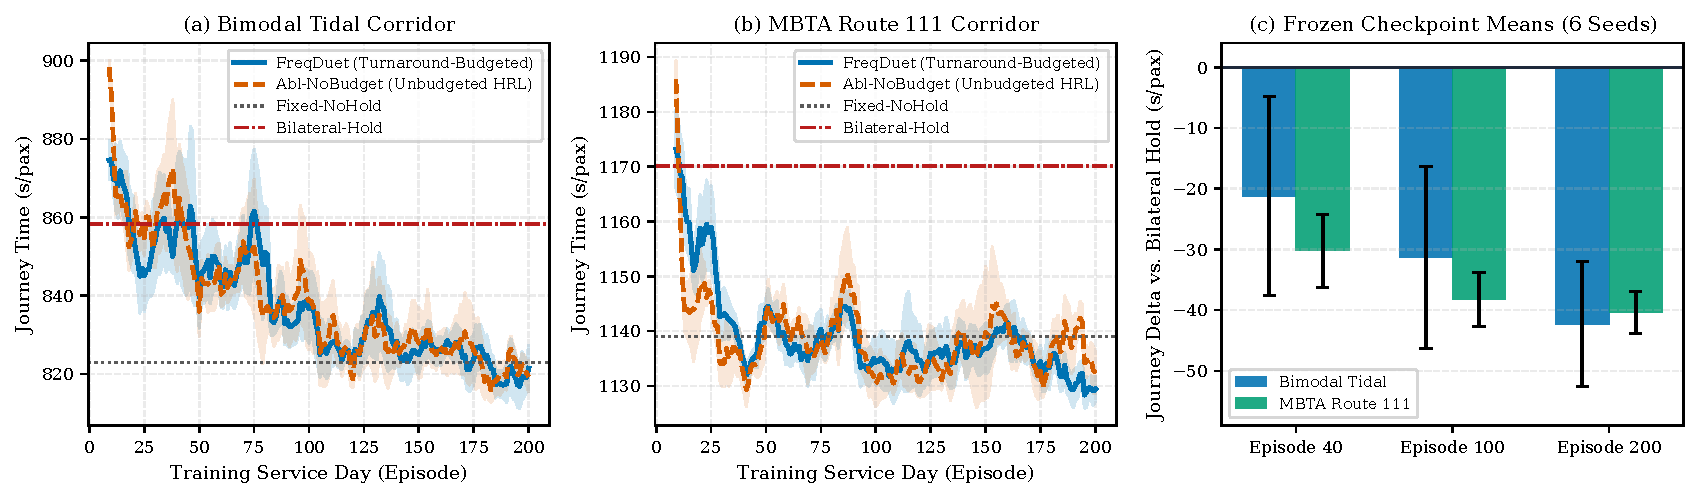
\includegraphics[width=\textwidth]{figures/fig3_stability_curves.pdf}
  \caption{Training-day journeys and frozen checkpoint performance. Panels (a,b) compare the nine-episode rolling means of six FreqDuet and four NoBudget seeds, with $\pm1$ standard error across seeds. Panel (c) uses the six FreqDuet seeds evaluated at three checkpoints on ten validation days, with between-seed SDs, relative to the fixed bilateral comparator. The training curves and frozen checkpoint means answer different questions.}
  \label{fig:stability}
\end{figure}

\begin{table}[!ht]
\centering\small
\caption{Validation at three frozen checkpoints in V501 (six training seeds and ten paired days). The $\pm$ term is the SD across seed-level means.}
\label{tab:checkpoints}
\begin{tabular}{@{}lrrrr@{}}
\toprule
Episode & $J$ (s/pax) & Wait (s/pax) & EWT (s) & Readiness (s/trip) \\
\RowsCheckpoints
\bottomrule
\end{tabular}
\end{table}

The pooled validation journey estimate decreases from episode 40 to 200 by 10.18~s/pax on MBTA-111 and 21.09~s/pax on Tidal-Bimodal (Table~\ref{tab:checkpoints}). This is not monotonic learning across seeds. From episode 100 to 200, the journey estimate deteriorates for one of six MBTA-111 seeds and two of six Tidal-Bimodal seeds. For example, on Tidal-Bimodal, seed 102 increases from 823.83 to 835.68~s/pax. The comparison of the six-seed and four-seed training curves (Figure~\ref{fig:stability}) is descriptive and does not establish that the ledger prevents late-training reversals.

\subsection{Demand Feature Comparisons}
\label{sec:results_ablation}

On MBTA-111, the aligned representation reduces journey exposure by 9.59~s/pax relative to the coarse-input NoFreq-HRL ($[-14.25,-5.50]$). All four matched seed-level differences favor FreqDuet (between $-15.82$ and $-4.44$~s/pax, averaging over test days within each seed). The advantages over RawHistory, AllBand and Swapped are smaller: their paired seed-by-day intervals include zero. The NoBudget and NoPromotion contrasts also include zero, although NoPromotion has a higher readiness delay point estimate on MBTA-111.

On Tidal-Bimodal, the direction changes: NoFreq-HRL, RawHistory and AllBand have lower journey point estimates than the aligned method. For example, FreqDuet minus NoFreq-HRL is $+8.24$~s/pax ($[-2.76,+22.41]$). The two corridors differ in load, geography and modeled traffic and demand, so this comparison cannot identify a signal-to-noise threshold or the cause of the reversal. Figure~\ref{fig:ablation} summarizes the feature and regularity comparisons.

\begin{figure}[!ht]
  \centering
  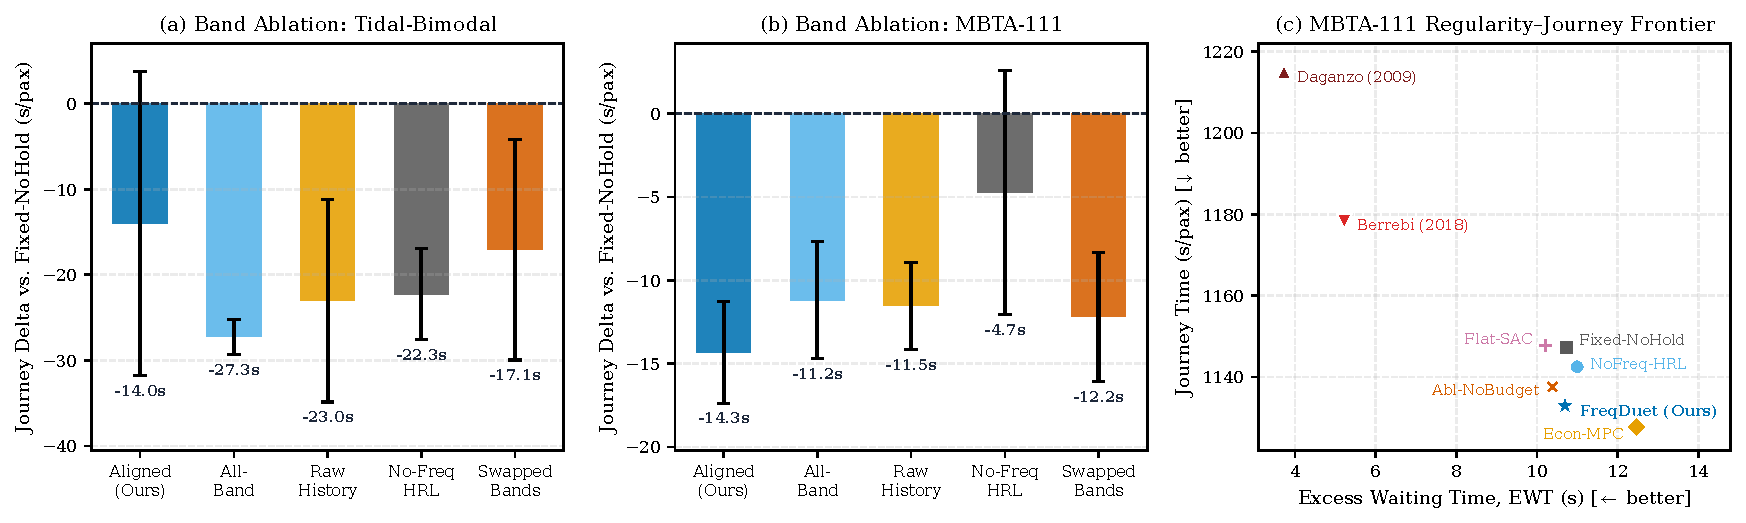
\includegraphics[width=\textwidth]{figures/fig4_frequency_budget_ablation.pdf}
  \caption{(a,b) Journey differences from Fixed-NoHold for five demand feature representations. Bars show between-seed SDs, not confidence intervals. (c) EWT relative to each controller's own target plan versus journey exposure for selected MBTA-111 controllers.}
  \label{fig:ablation}
\end{figure}

\subsection{Perturbed Demand, Running Speeds and Stationary Transfer}
\label{sec:results_ood}

On MBTA-111, FreqDuet has lower journey point estimates than Fixed-NoHold under all three perturbations. Other learned variants also improve in all three, and the ranking relative to alternatives changes. Under congestion, FreqDuet reduces journey exposure by 28.16~s/pax and readiness delay by 78.73~s/trip relative to the Rolling-Heuristic. Against Fixed-NoHold on that same cohort, it reduces journey exposure by 7.68~s/pax but increases readiness delay from 10.41 to 13.81~s/trip. On Tidal-Bimodal, the journey gain over the Rolling-Heuristic under congestion is 4.96~s/pax, and several feature variants have better journey point estimates than the aligned method. With a shifted tidal peak, FreqDuet averages 1.62~s/pax more journey exposure than Fixed-NoHold. These are regime-specific contrasts, not evidence of general robustness across routes.

\begin{figure}[!ht]
  \centering
  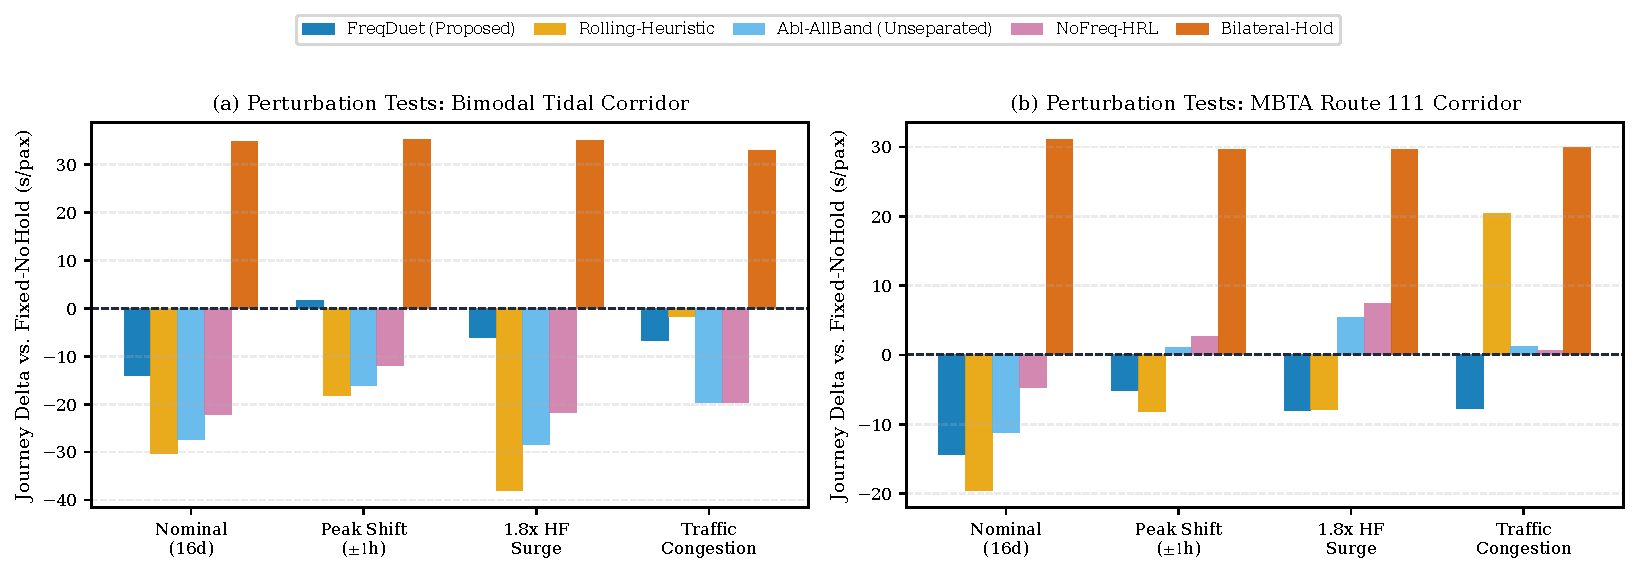
\includegraphics[width=\textwidth]{figures/fig5_ood_generalization.pdf}
  \caption{Journey differences from Fixed-NoHold in the nominal and three perturbed regimes for selected policies. Differences are point estimates on paired simulated days; negative values favor the indicated policy.}
  \label{fig:ood}
\end{figure}

\begin{table}[!ht]
\centering\small
\caption{Perturbation results on eight matched days per regime and corridor. $J$ is restricted journey exposure (s/pax), and $D$ is readiness delay (s/trip).}
\label{tab:ood_stress}
\begin{tabular}{@{}lrrrrrr@{}}
\toprule
 & \multicolumn{2}{c}{Peak shift} & \multicolumn{2}{c}{Local surges} & \multicolumn{2}{c}{Slower running} \\
\cmidrule(lr){2-3}\cmidrule(lr){4-5}\cmidrule(l){6-7}
Controller & $J$ & $D$ & $J$ & $D$ & $J$ & $D$ \\
\RowsOod
\bottomrule
\end{tabular}
\end{table}

The stationary test (Table~\ref{tab:transfer}) transfers only the Tidal-Bimodal learned policies. Compared with Fixed-NoHold, FreqDuet has longer journeys by 106.40~s/pax and greater readiness delay by 26.12~s/trip. It outperforms some other dynamic policies but does worse than the fixed policy on both outcomes. The Flat-Null development probe used non-learning rules; it is not an in-domain learned control for this transfer.

\begin{table}[!ht]
\centering\small
\caption{Flat-Null transfer from Tidal-Bimodal (eight paired days). Learned controllers are frozen. $\Delta J$ is FreqDuet minus the indicated comparator with a pointwise 95\% seed-by-day bootstrap interval. No MBTA-111 policy was evaluated on this transfer.}
\label{tab:transfer}
\begin{tabular}{@{}lrrr@{}}
\toprule
Controller & $J$ (s/pax) & $D$ (s/trip) & $\Delta J$ (s/pax) \\
\RowsTransfer
\bottomrule
\end{tabular}
\end{table}
